% Include from the paper/ directory. Tables already contain table environments.
% Requires booktabs. Synthetic Mini-200 only; not OPV2V acceptance.

% Cells copied from experiments/registry.csv. Selection: last no_communication or loss_dropped row for B0, B1, B2, B3, and B4. git_commit values in those rows: 04ee1ba.
\begin{table}[t]
\centering
\caption{Synthetic Mini-200 gate rows copied from the registry. Each cell is the last \texttt{no\_communication} or \texttt{loss\_dropped} row of that method. This is not acceptance on real OPV2V.}
\label{tab:gate3}
\scriptsize
\setlength{\tabcolsep}{3pt}
\begin{tabular}{lllllllll}
\toprule
method & bytes & mbps at 10 Hz & mIoU & vehicle IoU & road IoU & unknown F1 & UFE & status \\
\midrule
B0 & 0 & 0 & 0 & 0 & 0 & 0.84751653 & 0 & no\_communication \\
B1 & 16384 & 1.31072 & 0.36326521 & 0.43390366 & 0.51785785 & 0.94645161 & 0.025969892 & loss\_dropped \\
B2 & 16384 & 1.31072 & 0.43361293 & 0.58892433 & 0.32930311 & 0.94667013 & 0.053487873 & loss\_dropped \\
B3 & 16384 & 1.31072 & 0.29434875 & 0.092169858 & 0.37177833 & 0.9594036 & 0.030232978 & loss\_dropped \\
B4 & 16384 & 1.31072 & 0.35221265 & 0.29825046 & 0.43330968 & 0.96020233 & 0.026472607 & loss\_dropped \\
\bottomrule
\end{tabular}
\end{table}


\begin{figure}[t]
\centering
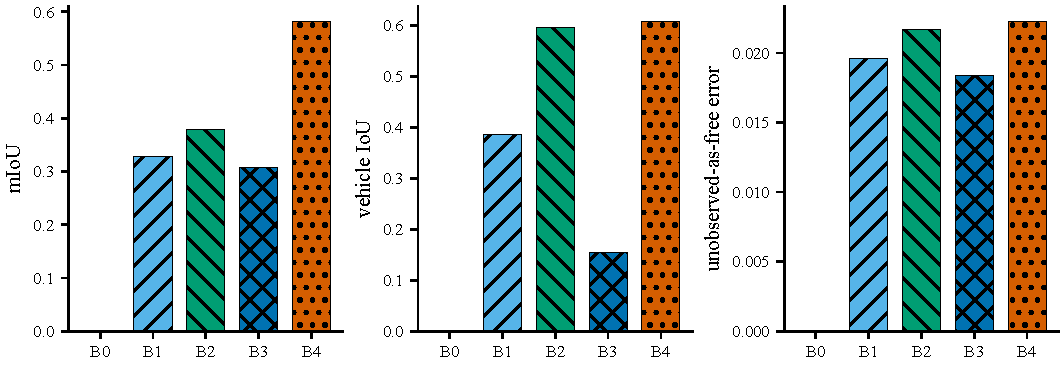
\includegraphics[width=0.95\textwidth]{figures/fig_gate3.pdf}
\caption{Synthetic Mini-200 gate comparison copied from the last matching rows of \texttt{experiments/registry.csv}. Bar heights are those cells. This is not acceptance on real OPV2V.}
\label{fig:gate3}
\end{figure}

% Cells copied from outputs/phase5/measurements.csv, family=bandwidth.
\begin{table}[t]
\centering
\caption{Synthetic Mini-200 \texttt{bandwidth} rows copied from \texttt{outputs/phase5/measurements.csv}. Empty CSV cells are left as --.}
\label{tab:bandwidth}
\scriptsize
\setlength{\tabcolsep}{3pt}
\begin{tabular}{llllllllll}
\toprule
method & level & bytes & bytes min & bytes max & mIoU & vehicle IoU & road IoU & unknown F1 & UFE \\
\midrule
B3 & 2048 & 2048 & 2048 & 2048 & 0.012338452 & 0.02825792 & 0 & 0.85851005 & 0.00064209755 \\
B3 & 4096 & 4096 & 4096 & 4096 & 0.048272822 & 0.034434621 & 0 & 0.8732753 & 0.0028373827 \\
B3 & 8192 & 8192 & 8192 & 8192 & 0.081184336 & 0.089026311 & 0.00018172732 & 0.89583984 & 0.0093892424 \\
B3 & 12288 & 12288 & 12288 & 12288 & 0.25302302 & 0.10987744 & 0.28839866 & 0.95559464 & 0.024179158 \\
B3 & 16384 & 16384 & 16384 & 16384 & 0.29434875 & 0.092169858 & 0.37177833 & 0.9594036 & 0.030232978 \\
B4 & 2048 & 2048 & 2048 & 2048 & 0.083772817 & 0.053219829 & 0 & 0.9111569 & 0.029825452 \\
B4 & 4096 & 4096 & 4096 & 4096 & 0.10480552 & 0.086280902 & 0 & 0.91546933 & 0.025589563 \\
B4 & 8192 & 8192 & 8192 & 8192 & 0.14242557 & 0.30793554 & 0 & 0.90912932 & 0.014540896 \\
B4 & 12288 & 12288 & 12288 & 12288 & 0.29453062 & 0.30692081 & 0.038667059 & 0.95042453 & 0.02014682 \\
B4 & 16384 & 16384 & 16384 & 16384 & 0.35221265 & 0.29825046 & 0.43330968 & 0.96020233 & 0.026472607 \\
\bottomrule
\end{tabular}
\end{table}


\begin{figure}[t]
\centering
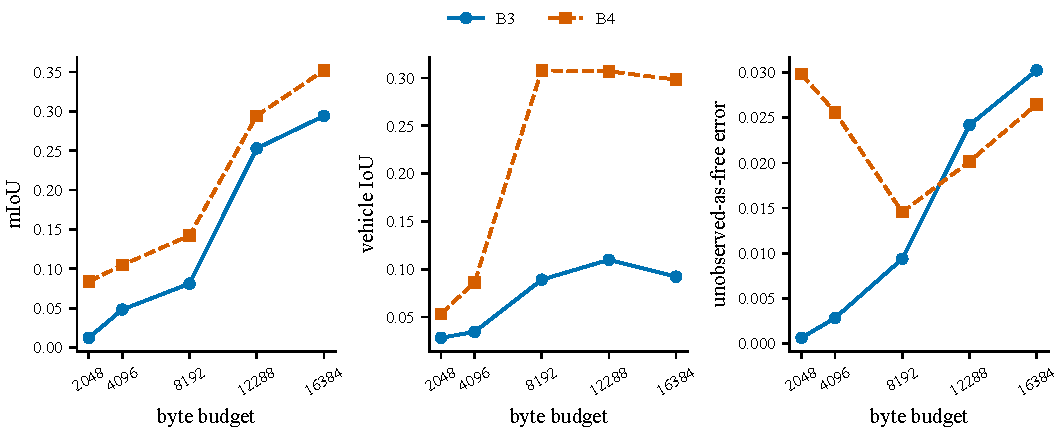
\includegraphics[width=0.95\textwidth]{figures/fig_bandwidth.pdf}
\caption{Synthetic Mini-200 \texttt{bandwidth} rows copied from \texttt{outputs/phase5/measurements.csv}. Tick labels are the CSV level strings.}
\label{fig:bandwidth}
\end{figure}

% Cells copied from outputs/phase5/measurements.csv, family=senders.
\begin{table}[t]
\centering
\caption{Synthetic Mini-200 \texttt{senders} rows copied from \texttt{outputs/phase5/measurements.csv}. Empty CSV cells are left as --.}
\label{tab:senders}
\scriptsize
\setlength{\tabcolsep}{3pt}
\begin{tabular}{llllllllll}
\toprule
method & level & bytes & bytes min & bytes max & mIoU & vehicle IoU & road IoU & unknown F1 & UFE \\
\midrule
B3 & 1 & 16384 & 16384 & 16384 & 0.15463547 & 0.015410637 & 0.32137886 & 0.90932123 & 0.015188518 \\
B3 & 2 & 16384 & 16384 & 16384 & 0.25528612 & 0.060375726 & 0.35500747 & 0.94794349 & 0.026854211 \\
B3 & 3 & 16384 & 16384 & 16384 & 0.29434875 & 0.092169858 & 0.37177833 & 0.9594036 & 0.030232978 \\
B4 & 1 & 16384 & 16384 & 16384 & 0.17669809 & 0.11244833 & 0.35501625 & 0.92685837 & 0.015413316 \\
B4 & 2 & 16384 & 16384 & 16384 & 0.2920871 & 0.22689267 & 0.36602784 & 0.952417 & 0.023624175 \\
B4 & 3 & 16384 & 16384 & 16384 & 0.35221265 & 0.29825046 & 0.43330968 & 0.96020233 & 0.026472607 \\
\bottomrule
\end{tabular}
\end{table}


\begin{figure}[t]
\centering
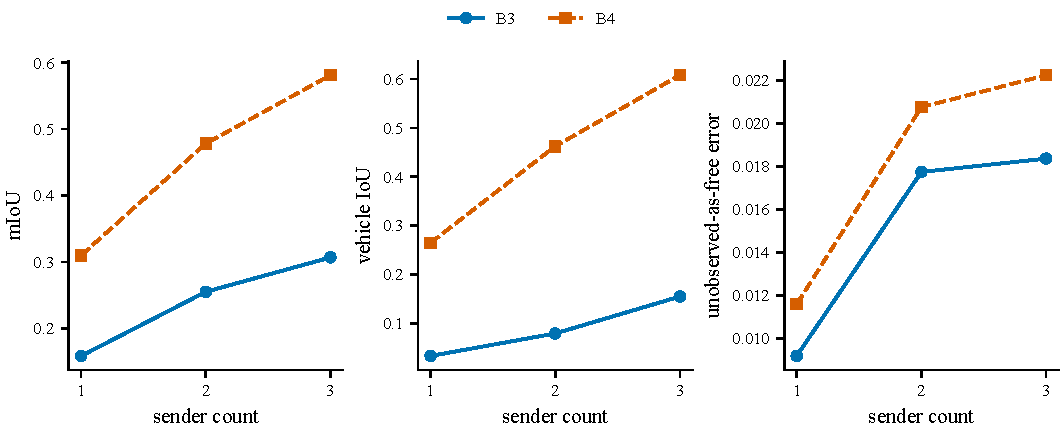
\includegraphics[width=0.95\textwidth]{figures/fig_senders.pdf}
\caption{Synthetic Mini-200 \texttt{senders} rows copied from \texttt{outputs/phase5/measurements.csv}. Tick labels are the CSV level strings.}
\label{fig:senders}
\end{figure}

% Cells copied from outputs/phase5/measurements.csv, family=weather.
\begin{table}[t]
\centering
\caption{Synthetic Mini-200 \texttt{weather} rows copied from \texttt{outputs/phase5/measurements.csv}. Empty CSV cells are left as --.}
\label{tab:weather}
\scriptsize
\setlength{\tabcolsep}{3pt}
\begin{tabular}{llllllllll}
\toprule
method & level & bytes & bytes min & bytes max & mIoU & vehicle IoU & road IoU & unknown F1 & UFE \\
\midrule
B3 & clear & 16384 & 16384 & 16384 & 0.30673264 & 0.15493385 & 0.53736162 & 0.96565475 & 0.01836076 \\
B3 & fog & 16384 & 16384 & 16384 & 0.20184488 & 0.11919204 & 0.42802703 & 0.94735829 & 0.011834822 \\
B3 & rain & 16384 & 16384 & 16384 & 0.26687793 & 0.090187891 & 0.48045167 & 0.96018005 & 0.014647983 \\
B4 & clear & 16384 & 16384 & 16384 & 0.58135053 & 0.60779025 & 0.64070693 & 0.97254069 & 0.022242667 \\
B4 & fog & 16384 & 16384 & 16384 & 0.4005961 & 0.53349453 & 0.59555573 & 0.96260723 & 0.014146969 \\
B4 & rain & 16384 & 16384 & 16384 & 0.44631922 & 0.34572079 & 0.30824727 & 0.96831071 & 0.023945012 \\
\bottomrule
\end{tabular}
\end{table}


\begin{figure}[t]
\centering
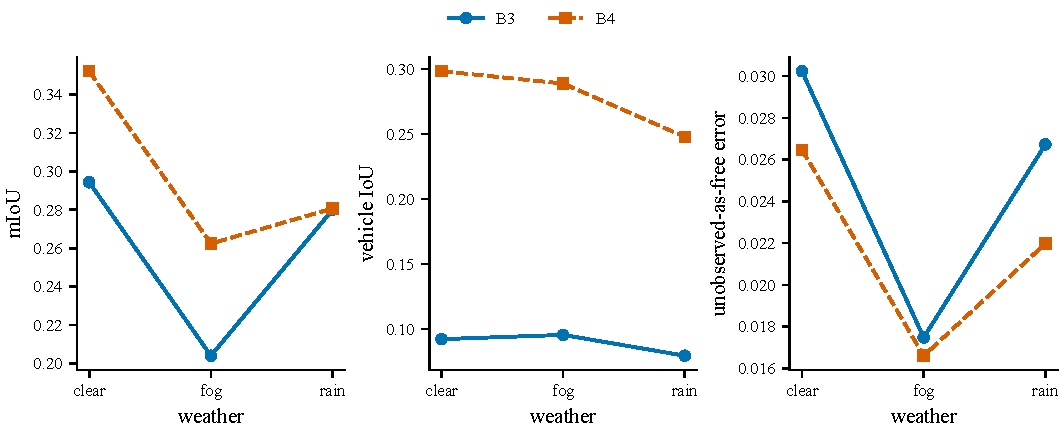
\includegraphics[width=0.95\textwidth]{figures/fig_weather.pdf}
\caption{Synthetic Mini-200 \texttt{weather} rows copied from \texttt{outputs/phase5/measurements.csv}. Tick labels are the CSV level strings.}
\label{fig:weather}
\end{figure}

% Cells copied from outputs/phase5/measurements.csv, family=pose.
\begin{table}[t]
\centering
\caption{Synthetic Mini-200 \texttt{pose} rows copied from \texttt{outputs/phase5/measurements.csv}. Empty CSV cells are left as --.}
\label{tab:pose}
\scriptsize
\setlength{\tabcolsep}{3pt}
\begin{tabular}{llllllllll}
\toprule
method & level & bytes & bytes min & bytes max & mIoU & vehicle IoU & road IoU & unknown F1 & UFE \\
\midrule
B3 & 0.0\_0.0 & 16384 & 16384 & 16384 & 0.29434875 & 0.092169858 & 0.37177833 & 0.9594036 & 0.030232978 \\
B3 & 0.5\_2.0 & 16384 & 16384 & 16384 & 0.22835025 & 0.081508945 & 0.36549788 & 0.95145709 & 0.037038957 \\
B3 & 1.0\_5.0 & 16384 & 16384 & 16384 & 0.1729324 & 0.055744313 & 0.32358541 & 0.94007342 & 0.045228994 \\
B4 & 0.0\_0.0 & 16384 & 16384 & 16384 & 0.35221265 & 0.29825046 & 0.43330968 & 0.96020233 & 0.026472607 \\
B4 & 0.5\_2.0 & 16384 & 16384 & 16384 & 0.25991842 & 0.22457027 & 0.42688299 & 0.9523199 & 0.028383601 \\
B4 & 1.0\_5.0 & 16384 & 16384 & 16384 & 0.19719875 & 0.15434963 & 0.37342614 & 0.94225854 & 0.034561081 \\
\bottomrule
\end{tabular}
\end{table}


\begin{figure}[t]
\centering
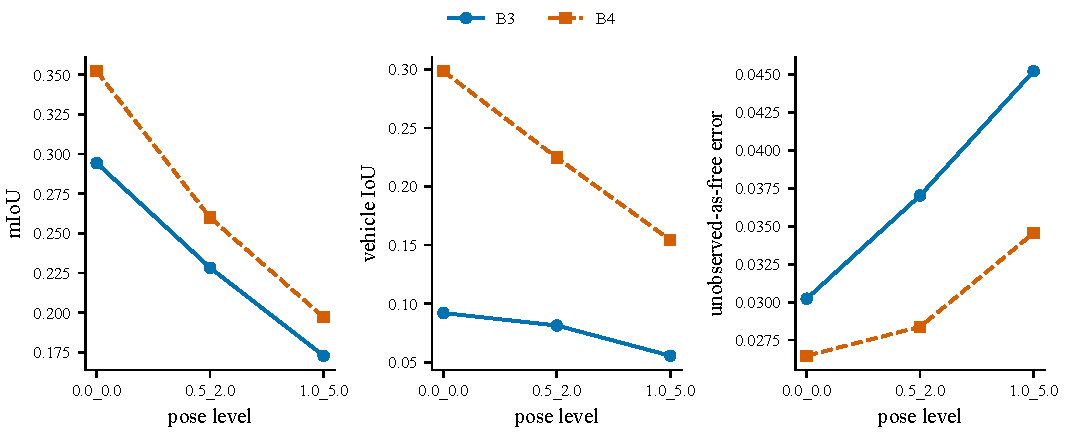
\includegraphics[width=0.95\textwidth]{figures/fig_pose.pdf}
\caption{Synthetic Mini-200 \texttt{pose} rows copied from \texttt{outputs/phase5/measurements.csv}. Tick labels are the CSV level strings.}
\label{fig:pose}
\end{figure}

% Cells copied from outputs/phase5/measurements.csv, family=latency.
\begin{table}[t]
\centering
\caption{Synthetic Mini-200 \texttt{latency} rows copied from \texttt{outputs/phase5/measurements.csv}. Empty CSV cells are left as --.}
\label{tab:latency}
\scriptsize
\setlength{\tabcolsep}{3pt}
\begin{tabular}{llllllllll}
\toprule
method & level & bytes & bytes min & bytes max & mIoU & vehicle IoU & road IoU & unknown F1 & UFE \\
\midrule
B3 & 0 & 16384 & 16384 & 16384 & 0.29434875 & 0.092169858 & 0.37177833 & 0.9594036 & 0.030232978 \\
B3 & 1 & 16384 & 16384 & 16384 & 0.27266022 & 0.068923378 & 0.35774818 & 0.95250976 & 0.02831221 \\
B3 & 2 & 16384 & 16384 & 16384 & 0.27797609 & 0.066748092 & 0.35807705 & 0.95266127 & 0.028445644 \\
B3 & 5 & 16384 & 16384 & 16384 & 0.25706565 & 0.040076222 & 0.32670955 & 0.9500902 & 0.028785603 \\
B4 & 0 & 16384 & 16384 & 16384 & 0.35221265 & 0.29825046 & 0.43330968 & 0.96020233 & 0.026472607 \\
B4 & 1 & 16384 & 16384 & 16384 & 0.32037436 & 0.20346839 & 0.40864291 & 0.95298934 & 0.024771112 \\
B4 & 2 & 16384 & 16384 & 16384 & 0.32707454 & 0.20259903 & 0.40868344 & 0.95357379 & 0.024735416 \\
B4 & 5 & 16384 & 16384 & 16384 & 0.30103485 & 0.114402 & 0.3476651 & 0.9512373 & 0.024958939 \\
\bottomrule
\end{tabular}
\end{table}


\begin{figure}[t]
\centering
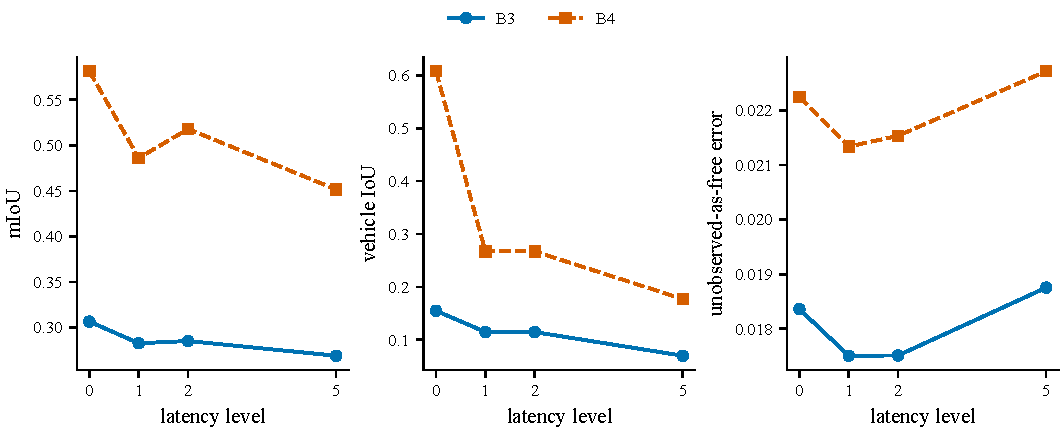
\includegraphics[width=0.95\textwidth]{figures/fig_latency.pdf}
\caption{Synthetic Mini-200 \texttt{latency} rows copied from \texttt{outputs/phase5/measurements.csv}. Tick labels are the CSV level strings.}
\label{fig:latency}
\end{figure}

% Cells copied from outputs/phase5/measurements.csv, family=packet_loss.
\begin{table}[t]
\centering
\caption{Synthetic Mini-200 \texttt{packet\_loss} rows copied from \texttt{outputs/phase5/measurements.csv}. Empty CSV cells are left as --.}
\label{tab:packet_loss}
\scriptsize
\setlength{\tabcolsep}{3pt}
\begin{tabular}{llllllllll}
\toprule
method & level & bytes & bytes min & bytes max & mIoU & vehicle IoU & road IoU & unknown F1 & UFE \\
\midrule
B3 & 0.0 & 16384 & 16384 & 16384 & 0.29434875 & 0.092169858 & 0.37177833 & 0.9594036 & 0.030232978 \\
B3 & 0.1 & 14678.333 & 13120 & 15976 & 0.27843444 & 0.08404033 & 0.35412647 & 0.95799195 & 0.028113759 \\
B3 & 0.25 & 12291.533 & 10536 & 14208 & 0.24975113 & 0.073323508 & 0.32153702 & 0.95515366 & 0.024797034 \\
B3 & 0.5 & 8162.8 & 6184 & 9992 & 0.18004533 & 0.047856615 & 0.22551604 & 0.94469119 & 0.017842748 \\
B4 & 0.0 & 16384 & 16384 & 16384 & 0.35221265 & 0.29825046 & 0.43330968 & 0.96020233 & 0.026472607 \\
B4 & 0.1 & 14747.467 & 13528 & 16112 & 0.32927958 & 0.27688038 & 0.40493756 & 0.95913145 & 0.025884903 \\
B4 & 0.25 & 12430.933 & 10672 & 13936 & 0.2928118 & 0.2444855 & 0.36078055 & 0.95682031 & 0.025464628 \\
B4 & 0.5 & 8439.3333 & 6048 & 10128 & 0.20946897 & 0.17309662 & 0.27644985 & 0.94994764 & 0.025567466 \\
\bottomrule
\end{tabular}
\end{table}


\begin{figure}[t]
\centering
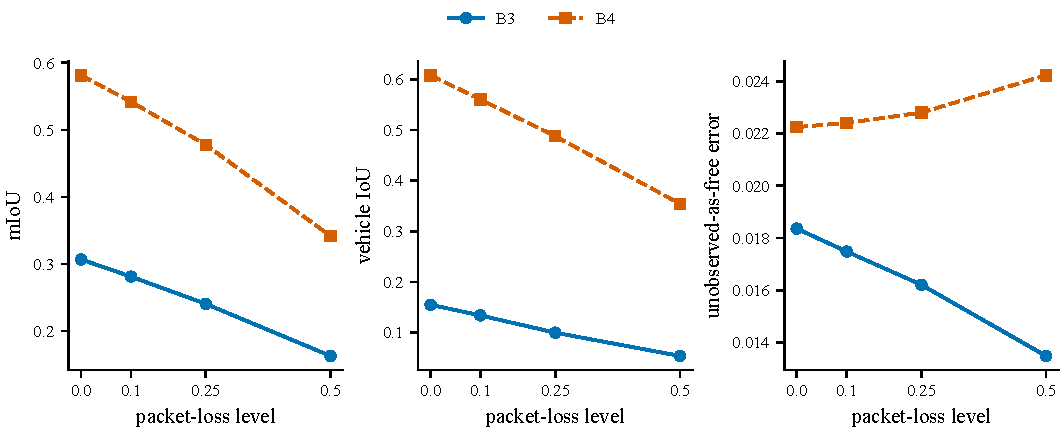
\includegraphics[width=0.95\textwidth]{figures/fig_packet_loss.pdf}
\caption{Synthetic Mini-200 \texttt{packet\_loss} rows copied from \texttt{outputs/phase5/measurements.csv}. Tick labels are the CSV level strings.}
\label{fig:packet_loss}
\end{figure}

% Cells copied from outputs/phase5/measurements.csv, family=seed.
\begin{table}[t]
\centering
\caption{Synthetic Mini-200 \texttt{seed} rows copied from \texttt{outputs/phase5/measurements.csv}. Empty CSV cells are left as --.}
\label{tab:seed}
\scriptsize
\setlength{\tabcolsep}{3pt}
\begin{tabular}{llllllllll}
\toprule
method & level & bytes & bytes min & bytes max & mIoU & vehicle IoU & road IoU & unknown F1 & UFE \\
\midrule
B3 & 0 & 16384 & 16384 & 16384 & 0.30673264 & 0.15493385 & 0.53736162 & 0.96565475 & 0.01836076 \\
B4 & 0 & 16384 & 16384 & 16384 & 0.58135053 & 0.60779025 & 0.64070693 & 0.97254069 & 0.022242667 \\
B3 & 1 & 16384 & 16384 & 16384 & 0.32210002 & 0.37351284 & 0.42498272 & 0.96585322 & 0.02167876 \\
B4 & 1 & 16384 & 16384 & 16384 & 0.51051915 & 0.49717663 & 0.58255527 & 0.96961605 & 0.028882491 \\
B3 & 2 & 16384 & 16384 & 16384 & 0.36913614 & 0.19934963 & 0.62242168 & 0.96523695 & 0.021541077 \\
B4 & 2 & 16384 & 16384 & 16384 & 0.52305851 & 0.48327883 & 0.61659821 & 0.97046287 & 0.019375963 \\
\bottomrule
\end{tabular}
\end{table}


\begin{figure}[t]
\centering
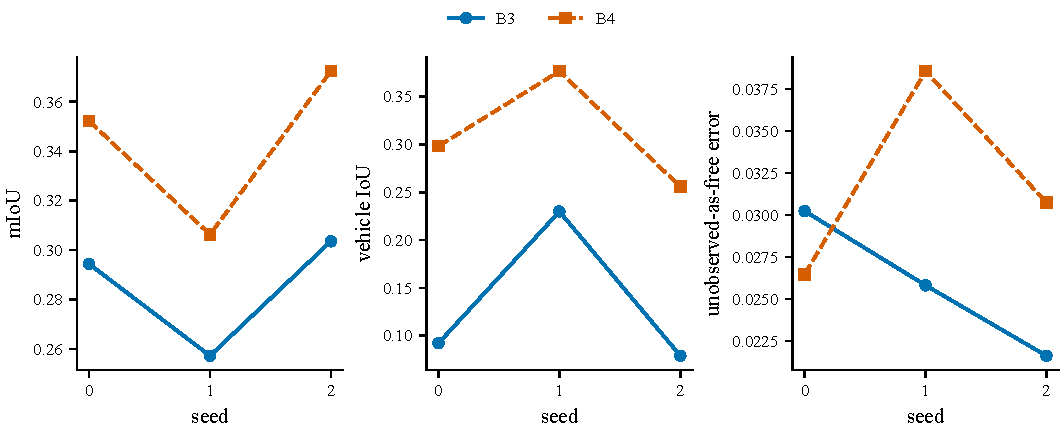
\includegraphics[width=0.95\textwidth]{figures/fig_seeds.pdf}
\caption{Synthetic Mini-200 \texttt{seed} rows copied from \texttt{outputs/phase5/measurements.csv}. Tick labels are the CSV level strings.}
\label{fig:seed}
\end{figure}

% Ablations were not run. This is not a result table.
% Reasons are copied from outputs/phase5/ablations.csv.
\paragraph{Ablations.}
These ablations were not run. No metric cells are filled.
\begin{itemize}
\item \texttt{envelope}: not\_run. B4 always writes the 512-byte envelope. There is no switch that removes it.
\item \texttt{grouped\_codebooks}: not\_run. Three geometry books versus one shared book is the B4 versus B3 pair, not a switch on one weight.
\item \texttt{road\_quota}: not\_run. The quota floors are fixed arguments. Changing them would be a new selection rule.
\item \texttt{second\_code\_level}: not\_run. Transmit defaults to stage 1, which is the stage the decoder was trained on.
\end{itemize}

